%% AMS-LaTeX Created by Wolfram Mathematica 9.0 : www.wolfram.com

\documentclass{article}
\usepackage{amsmath, amssymb, graphics, setspace}
\usepackage{graphicx}
\usepackage{xcolor}
\usepackage{hyperref}
\usepackage{tikz}
\usepackage[utf8]{inputenc}
\usepackage{spverbatim}
\usepackage{geometry}
 \geometry{
 a4paper,
 left=15mm,
 right=10mm,
 top=20mm,
 bottom=20mm,
 }

\DeclareMathSizes{10}{10}{10}{10}

\newcommand{\mathsym}[1]{{}}
\newcommand{\unicode}[1]{{}}

\newcounter{mathematicapage}
\begin{document}


\section{Ampliación 2D}
\subsection{Cambios  en el código}


\paragraph{Esquemas numéricas implementadas}  

\begin{description}
\item  parámetro schemeType en constants.py
\item las mismas esquemas de 1D extendidas  a 2D
\item \textbf{LF}
\item un solo paso de tiempo: FTCS usando en lugar de $u_{i,j}$ la media espacial
\item \textbf{Lax Wendroff} 
\item 2 pasos de tiempo: el primero LF y el segundo Leapfrog
\item como los elementos de la matriz fc de dimension 2x2 (para cada punto de la red)
 $f_{0,1} = f_{1,0}$  guardo para cada punto un array de 3 elementos $(p+\rho v_x^2, \rho v_x v_y, p+\rho v_y^2)$
\item 2 implementaciones


\item Lax Wendroff 1
\begin{figure}[ht]
  \centering
		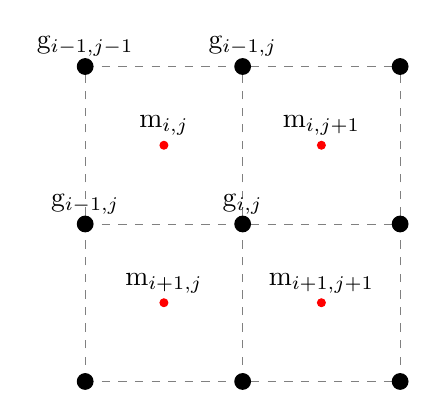
\begin{tikzpicture}

    \draw[style=help lines,dashed] (-0.001,-0.001) grid[step=2cm] (4,4);
          % Draws a grid in the new coordinates.
          %\filldraw[fill=gray, fill opacity=0.3, draw=black] (0,0) rectangle (2,2);
              % Puts the shaded rectangle
    \foreach \x in {0,...,2}{% Two indices running over each
      \foreach \y in {0,...,2}{% node on the grid we have drawn 
        \node[draw,circle,inner sep=2pt,fill] at (2*\x,2*\y) {};
            % Places a dot at those points
      }
    }

		\node[draw,red,circle,inner sep=1pt,fill] at (1,3) {};
		\node[above] at (1,3) {m$_{i,j}$};
		\node[draw,red,circle,inner sep=1pt,fill] at (3,3) {};
		\node[above] at (3,3) {m$_{i,j+1}$};
		\node[draw,red,circle,inner sep=1pt,fill] at (1,1) {};
		\node[above] at (1,1) {m$_{i+1,j}$};
		\node[draw,red,circle,inner sep=1pt,fill] at (3,1) {};
		\node[above] at (3,1) {m$_{i+1,j+1}$};

		\node[above] at (0,4) {g$_{i-1,j-1}$};
		\node[above] at (2,4) {g$_{i-1,j}$};
		\node[above] at (0,2) {g$_{i-1,j}$};
		\node[above] at (2,2) {g$_{i,j}$};


		\end{tikzpicture}


  \caption{lw}
  \label{lw}
\end{figure}

\item en esta implementación se calcula un solo array de puntos intermedios
\item en el primer paso se calcula u en los puntos intermedios $m_{i,j}$

\item para las variables ue, um (escalares):
\item $u_{m_{i,j}} = \frac{1}{4}  (u_{g_{i-1,j-1}} + u_{g_{i-1,j}} + u_{g_{i,j-1}} + u_{g_{i,j}}) - \frac{1}{4}\big[
\frac{dt}{dz_0} (f_{g_{i,j},0} - f_{g_{i-1,j},0} + f_{g_{i,j-1},0} - f_{g_{i-1,j-1},0} ) +
\frac{dt}{dz_1} (f_{g_{i,j},1} - f_{g_{i,j-1},1} + f_{g_{i-1,j},1} - f_{g_{i-1,j-1},1} )  \big] $
\item para la variables uc (vector) ():
\item $u_{m_{i,j},0} = \frac{1}{4}  (u_{g_{i-1,j-1},0} + u_{g_{i-1,j},0} + u_{g_{i,j-1},0} + u_{g_{i,j},0}) - \frac{1}{4}\big[
\frac{dt}{dz_0} (f_{g_{i,j},0} - f_{g_{i-1,j},0} + f_{g_{i,j-1},0} - f_{g_{i-1,j-1},0} ) +
\frac{dt}{dz_1} (f_{g_{i,j},1} - f_{g_{i,j-1},1} + f_{g_{i-1,j},1} - f_{g_{i-1,j-1},1} )  \big] $
\item $u_{m_{i,j},1} = \frac{1}{4}  (u_{g_{i-1,j-1},1} + u_{g_{i-1,j},1} + u_{g_{i,j-1},1} + u_{g_{i,j},1}) - \frac{1}{4}\big[
\frac{dt}{dz_0} (f_{g_{i,j},1} - f_{g_{i-1,j},1} + f_{g_{i,j-1},1} - f_{g_{i-1,j-1},1} ) +
\frac{dt}{dz_1} (f_{g_{i,j},2} - f_{g_{i,j-1},2} + f_{g_{i-1,j},2} - f_{g_{i-1,j-1},2} )  \big] $

\item leapfrog en el segundo paso: se calcula u en los puntos $g_{i,j}$
\item para las variables ue, um :
\item  $u_{g_{i,j}} = u_{g_{i,j}} - \frac{1}{2} dt  \big[ \frac{1}{dz_0} (f_{m_{i+1,j},0} - f_{m_{i,j},0} + 
f_{m_{i+1,j+1},0} - f_{m_{i,j+1},0} )  +  \frac{1}{dz_1}
(f_{m_{i,j+1},1} - f_{m_{i,j},1} + f_{m_{i+1,j+1},1} - f_{m_{i+1,j},1}) \big] $
\item para la variable uc:
\item  $u_{g_{i,j},0} = u_{g_{i,j},0} - \frac{1}{2} dt  \big[ \frac{1}{dz_0} (f_{m_{i+1,j},0} - f_{m_{i,j},0} + 
f_{m_{i+1,j+1},0} - f_{m_{i,j+1},0} )  +  \frac{1}{dz_1}
(f_{m_{i,j+1},1} - f_{m_{i,j},1} + f_{m_{i+1,j+1},1} - f_{m_{i+1,j},1}) \big] $
\item  $u_{g_{i,j},1} = u_{g_{i,j},1} - \frac{1}{2} dt  \big[ \frac{1}{dz_0} (f_{m_{i+1,j},1} - f_{m_{i,j},1} + 
f_{m_{i+1,j+1},1} - f_{m_{i,j+1},1} )  +  \frac{1}{dz_1}
(f_{m_{i,j+1},2} - f_{m_{i,j},2} + f_{m_{i+1,j+1},2} - f_{m_{i+1,j},2}) \big] $


\newpage





\item Lax Wendroff 2

\begin{figure}[ht]
  \centering
		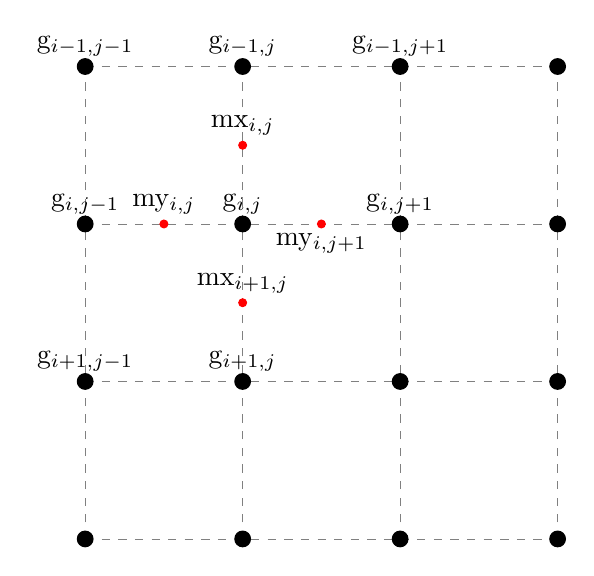
\begin{tikzpicture}


    \draw[style=help lines,dashed] (-0.001,-0.001) grid[step=2cm] (6,6);
          % Draws a grid in the new coordinates.
          %\filldraw[fill=gray, fill opacity=0.3, draw=black] (0,0) rectangle (2,2);
              % Puts the shaded rectangle
    \foreach \x in {0,...,3}{% Two indices running over each
      \foreach \y in {0,...,3}{% node on the grid we have drawn 
        \node[draw,circle,inner sep=2pt,fill] at (2*\x,2*\y) {};
            % Places a dot at those points
      }
    }

		\node[draw,red,circle,inner sep=1pt,fill] at (2,5) {};
		\node[above] at (2,5) {mx$_{i,j}$};
		\node[draw,red,circle,inner sep=1pt,fill] at (1,4) {};
		\node[above] at (1,4) {my$_{i,j}$};
		\node[draw,red,circle,inner sep=1pt,fill] at (2,3) {};
		\node[above] at (2,3) {mx$_{i+1,j}$};
		\node[draw,red,circle,inner sep=1pt,fill] at (3,4) {};
		\node[below] at (3,4) {my$_{i,j+1}$};

		\node[above] at (2,4) {g$_{i,j}$};
		\node[above] at (2,6) {g$_{i-1,j}$};
		\node[above] at (2,2) {g$_{i+1,j}$};
		\node[above] at (0,4) {g$_{i,j-1}$};
		\node[above] at (0,6) {g$_{i-1,j-1}$};
		\node[above] at (0,2) {g$_{i+1,j-1}$};
		\node[above] at (4,4) {g$_{i,j+1}$};
		\node[above] at (4,6) {g$_{i-1,j+1}$};
		\end{tikzpicture}


  \caption{lw2}
  \label{lw2}
\end{figure}

\item para las variables ue, um (escalares):
\item en el primer paso se calcula u en 2 arrays de  puntos intermedios $mx_{i,j}$ y $my_{i,j}$

\item $u_{mx_{i,j}} = \frac{1}{2}  (u_{g_{i-1,j}} + u_{g_{i,j}} ) - \big[
\frac{1}{8}\frac{dt}{dz_1} (f_{g_{i,j+1},1} - f_{g_{i,j-1},1} + f_{g_{i-1,j+1},1} - f_{g_{i-1,j-1},1} ) +
\frac{1}{2}\frac{dt}{dz_0} ( f_{g_{i,j},0} - f_{g_{i-1,j},0}  ) \big]  $

\item $u_{my_{i,j}} = \frac{1}{2}  (u_{g_{i,j-1}} + u_{g_{i,j}} ) - \big[
\frac{1}{8}\frac{dt}{dz_0} (f_{g_{i+1,j},0} - f_{g_{i-1,j},0} + f_{g_{i+1,j-1},0} - f_{g_{i-1,j-1},0} ) +
\frac{1}{2}\frac{dt}{dz_1} ( f_{g_{i,j},1} - f_{g_{i,j-1},1}  ) \big]  $
\item en el segundo paso:


\item $u_{g_{i,j}} =  u_{g_{i,j}} - \big[
   \frac{dt}{dz_0}  (f_{mx_{i+1,j},0} - f_{mx_{i,j},0} )+ 
   \frac{dt}{dz_1}  (f_{my_{i,j+1},1} - f_{my_{i,j},1} ) 
\big]$ 

\item de forma similar se calcula para uc


\end{description}
\paragraph{Condiciones iniciales}
\begin{description}
\item la función de la perturbación(h) es ahora función de 2 variables(argFunc en perturbation\_params.py)  y la velocidad tiene 2 componentes
\item argFunc puede ser una función lineal de $x_0$ y $x_1$ (en perturbatoin\_params waveType = "lineal") o radial (en este caso la perturbación de la velocidad se genera a partir del gradiente de la función de perturbación y la densidad y presión  de tal forma que cumplan las relaciones de las amplitudes)

\end{description}
\paragraph{Visualización}
\begin{description}
\item los valores de las  variables que quiero representar (p, $\rho$ , v) son ahora arrays 2D y la velocidad tiene 2 componentes. Los dibujo como imagen y también puedo representar proyecciones de los valores en las 2 direcciones o en una dirección cualquiera
\item en el caso "wavepacket" dibujo la trayectoria calculada de forma analítica por encima de la imagen actual o también la puedo mostrar aparte (util por si está mal calculada! y luego no tengo que rehacer todo el calculo numérico )
\end{description}
	
\subsection{Tests}

\begin{description}
\item waveType = "lineal": el cartón en la dirección horizontal(argType="y"), vertical(argType="x"), diagonal(argType="d1") con functionType="sine" , "gauss" , "wavepacket\_carton"  y "wavepacket"
\item Intenté waveType="radial" con functionType="hankel" pero no salió muy bien
\end{description}


\subsection{Breve resumen de la teoria de ray tracing}
\begin{description}
\item Después de hacer unos cálculos de las ecuaciones de los fluidos (y suponiendo el caso general inhomogeneo en tiempo y espacio : 
$\rho_0 = \rho_0(x,t),p_0 = p_0(x,t) \implies c_s = c_s(x,t)$ 
con  $p_0, \rho_0, c_s$  monótonas, variando bastante lentamente en el espacio y tiempo de tal forma que se pueden omitir terminos de segundo orden o mas en multiplicaciones de derivadas temporales o espaciales de estas y las perturbaciones) las perturbaciones de las variables verifican las ecuaciones: 

\item $\frac{\partial}{\partial t} \big(\frac{1}{c_s^{2}(x,t)} \frac{\partial p\prime}{\partial t}\big) = \nabla^{2} p\prime    $
\item $\frac{\partial}{\partial t} \big(\frac{1}{c_s^{2}(x,t)} \frac{\partial \rho\prime}{\partial t}\big) = \nabla^{2} \rho\prime    $
\item $\frac{\partial}{\partial t} \big(\frac{1}{c_s^{2}(x,t)} \frac{\partial \Phi}{\partial t}\big) = \nabla^{2} \Phi $ donde definimos  $v = \nabla \Phi$ considerando el fluido irrotacional

\end{description}  

\paragraph{Medio homogéneo}

\begin{description}  
\item Si la densidad y presión de equilibrio son constantes en tiempo y espacio ($\rho_0, p_0 constantes \implies c_s const$) :
\item $\frac{1}{c_s^{2}} \frac{\partial^{2} p\prime}{\partial t^{2}} = \nabla^{2} p\prime    $
\item $\frac{1}{c_s^{2}} \frac{\partial^{2} \rho\prime}{\partial t^{2}} = \nabla^{2} \rho\prime    $
\item $\frac{1}{c_s^{2}} \frac{\partial^{2} \Phi}{\partial t^{2}} = \nabla^{2} \Phi    $
\item En 2d  la solución general es similar caso 1d de forma $F(k\cdot x+ \omega t) + G(k \cdot x- \omega t)$ con F, G funciones arbitrarias y  k y $\omega$ cumpliendo la relación de dispersión: $\omega = c_s |k|$ 
( por la T. Fourier F y G se pueden escribir como superposiciones de ondas harmónicas) 

\end{description}  


\paragraph{Medio inhomogéneo independiente de tiempo} $p_0 = p_0(x),\rho_0 = \rho_0(x)\implies c_s = c_s(x)$ monótonas, variando lentamente..
\begin{description}  
\item $\frac{1}{c_s^{2}(x)} \frac{\partial^{2} p\prime}{\partial t^{2}} = \nabla^{2} p\prime    $
\item $\frac{1}{c_s^{2}(x)} \frac{\partial^{2} \rho\prime}{\partial t^{2}} = \nabla^{2} \rho\prime    $
\item $\frac{1}{c_s^{2}(x)} \frac{\partial^{2} \Phi}{\partial t^{2}} = \nabla^{2} \Phi    $
\item Análogo a la solución del caso homogeneo de la onda plana:
 $p(x,t)=a cos(\phi(x))$ donde $\phi(x,t) = k\cdot x-\omega t$ con la amplitud a const y $\omega, k$ constantes verificando la relación de dispersión $\omega^{2} = c_s^2 k^2  $ intentamos  buscar soluciones de forma $a(x,t) e^{i\phi(x,t)}$ (aproximación WKB): 
 donde definimos 
\item $\omega(x,t) = -\frac{\partial \phi}{\partial t}$
\item $k(x,t) = -\nabla \phi$
\end{description}


\paragraph{Resolver la ecuación genérica}
\begin{description}  
\item $\frac{1}{c_s^{2}(x)} \frac{\partial^{2} p}{\partial t^{2}} = \nabla^{2} p  $
\item Reemplazando la solución WKB approx. $p(x,t) = a(x,t) e^{i \phi(x,t)}$ en la ecuación y con las definiciones de $\omega$ y k de arriba despues 
de hacer los cálculos 
y asumiendo  que las variaciones en la amplitud son muy pequeñas de forma que podemos omitir términos de segundo orden en las derivadas espaciales y temporales de a llegamos a: 
\begin{itemize}
\item $\omega^{2}(x,t) = c_s^{2}(x) k^2(x,t)$ (la relación de dispersión es válida de forma local)
\item y la ecuación de la evolución de la amplitud:
  $\frac{\partial a}{\partial t} + c_g \cdot \nabla a = -\frac{1}{2} \frac{a}{|k| c_s} (\frac{\partial \omega}{\partial t} + c_s^{2}  \nabla \cdot k) $
\end{itemize}
\item con $c_g = \frac{\partial \omega}{\partial k} = c_s \frac{k}{|k|}$ (k es un vector)  

\item de la relación de dispersión $\implies $ 
\item$\frac{\partial \omega}{\partial t} + c_g \cdot \nabla \omega = 0 $
\item$\frac{\partial k}{\partial t} + c_g \cdot \nabla k = -k \cdot \nabla  c_g $
\item$\frac{\partial \phi}{\partial t} + c_g \cdot \nabla \phi = 0 $

\item Usamos directamente la ecuación de conservación de energía para determinar la amplitud y no la de arriba (TODO):
\item$\frac{\partial E}{\partial t} + c_g \cdot \nabla E = -E \nabla \cdot c_g $

\end{description}


Al largo de un rayo  $x_p(t)$ solución de :

\begin{description}  
\item$\frac{dx}{dt} = c_g $
\item$ x(0) = x_p $
\end{description}
las dependencias de x se transforman en dependencias de t reemplazando x por $x_p(t) $ 

y reemplazando en las ecuaciones de arriba obtenemos  las ecuaciones diferenciales:
\begin{description}  
\item $\frac{d\omega}{dt} = 0$
\item $\frac{d\phi}{dt} = 0$
\item $\frac{dk}{dt} = -k \cdot \nabla c_g $
\item $\frac{da}{dt} = -\frac{1}{2} \frac{a}{|k| c_s} (\frac{\partial \omega}{\partial t} + c_s^{2}  \nabla \cdot k) $
\item$\frac{dE}{dt} = -E \nabla \cdot c_g $

\end{description}

\paragraph 2D

\begin{description}  
\item Las caracteristicas:
$\frac{dx_i}{dt} = c_s \frac{k_i}{\sqrt{k_0^2 + k_1^2}} $,  $i \in 0,1$
\item $\frac{d\omega}{dt} = 0 $
\item $\frac{dk_i}{dt} = -\frac{\partial c_s}{\partial x_i} |k| $,  $i \in 0,1$

\item Consideramos el caso inhomogeneo solo en una dirección: (considerando la dirección $e_0$, y es lo mismo para una dirección arbitraria cambiando el sistema de coordenadas, $c_s(x) = c_s(x_0) $)
\item $\frac{dk_1}{dt} = 0 $
\item $\frac{dk_0}{dt} = -\frac{\partial c_s}{\partial x_0} |k| $

\end{description}


al largo del rayo $x_p(t)$:
\begin{description}
\item $ \omega(x_p(t), t)  = constant $
\item $\phi(x_p(t),t) = constant$
\item $k_1(x_p(t),t) = constant$
\end{description}

\textbf{Relación entre las amplitudes} de las variables $p, \rho, v$ 

\begin{description}  
\item Suponiendo que estas soluciones existen:
\item $p\prime = P e^{i\phi}$
\item $\rho\prime = R e^{i\phi}$
\item $v = V e^{i\phi}$
\item P,R,V  complejos
\item de la relación de adiabaticidad: $|P(x,t)| = c_s^{2}(x) |R(x,t)|$
\item de la ecuación de movimiento: 
\item $\rho_0 \frac{\partial v}{\partial t} = -\nabla \rho\prime \implies -i \rho_0 \omega V e^{i\phi} = i k P e^{i\phi}$
\item despues de simplificar,  multiplicar cada lado con su conjugado(hay que expresar las amplitudes locales con el módulo porque pueden ser complejas):
\item  $|V|^2 = \frac{|P|^2}{\rho_0^{2} c_s^2} \implies$ 
\item $|V|= \frac{1}{c_s \rho_0} |P| = \frac{c_s}{p_0 \gamma} |P|$ 

\item es independiente de si el medio es homogéneo o no 
\item es independiente del número de dimensiones

\end{description}  

\section*{Practica}


\paragraph{Condiciones iniciales}	
\begin{description}
\item Definimos una amplitud A(en soundwave\_perturbation\_params.py) muy pequeña y una función periodica h en el intervalo $[x0_0, xf_0] x [x0_1, xf_1]$ (estos están en constants.py) con amplitud máxima 1 y creeamos las perturbaciones para que cumplan las relaciones entre las amplitudes de arriba y considerando una onda que empieza a propagarse en la dirección definida por la recta $n_x x - n_y y = 0$
\item definimos $ k_0 = \frac{n_x}{xf_0 - x0_0}, k_1 =  \frac{n_y}{xf_1 - x0_1}$ 
\item  $p\prime(x,0) = A \gamma p_0 h(x) $ 
\item  $\rho\prime(x,0) = A \rho_0 h(x) $
\item  $v(x, 0) =  A c_s h(x) (\frac{k_0}{|k|} , \frac{k_1}{|k|}) $ donde $|k| = \sqrt{k_0^2 + k_1^2} $
\item para el paquete de ondas (para el caso de propagación diagonal):
\begin{center}
\item $h(x) = e^{- \frac{(x_0-xc_0)^2 + (x_1 - xc_1)^2 }{W^2}} cos\big[2 \pi  K_0 (k_0(x_0 - x0_0) +  k_1(x_1 - x0_1)) \big] $
\end{center}
\end{description}

\paragraph{Fourier}

\begin{description}
\item reemplazo los parámetros $k_0$ y $k_1$ (multiplicándolos por $2 \pi K_0$) para escribir $ h(x) = e^{- \frac{(x_0-xc_0)^2 + (x_1 - xc_1)^2 }{W^2}} cos\big[k_0(x_0 - x0_0) +  k_1(x_1 - x0_1)) \big]  $
\item para el caso 1d $h_1(x) = e^{-\frac{(x-x_c)^2}{W^2} } cos(k_0(x-x_0)) $ 

\item había obtenido con mathematica (de forma analítica) la transformada fourier de h con FourierTransform sin especificar FourierParameters que por defecto son  $0, 1$  y obtengo $f_3(k)$. De la documentación de mathematica y también se puede comprobar de forma analítica y numérica $f_3(k) = \sqrt{\frac{1}{2 \pi}} \int_{- \infty}^{\infty}{h(x) e^{i k x} dx} $ 
\item después de hacer unos cálculos:
\item $f_3(k) = \frac{W}{2 \sqrt{2}}  e^{-i  k  x_c}  (u_1(k) + u_2(k)) $
\item $u_1(k) = e^{-\frac{W^2}{4}  (k+k_0)^2} e^{-i  k_0 (x_0-x_c)} $ 
\item $u_2(k) = e^{-\frac{W^2}{4}  (k-k_0)^2} e^{i  k_0 (x_0-x_c)} $ 
\item Uso esta  transf fourier para calcular en el caso 2d:
\item La transf fourier de $h(x_0, x_1)$ es 
\item $f_2(m,n) = \sqrt{\frac{1}{2 \pi}} \int_{- \infty}^{\infty}\int_{- \infty}^{\infty}{h(x_0,x_1) e^{i m x_0} e^{i n x_1} dx_0 dx_1 } $
\item $ =  \int_{- \infty}^{\infty}\int_{- \infty}^{\infty} {e^{- \frac{(x_0-xc_0)^2}{W^2}} 
e^{- \frac{(x_1-xc_1)^2}{W^2}}  cos\big[k_0(x_0 - x0_0) +  k_1(x_1 - x0_1)) \big] e^{i m x_0} e^{i n x_1} 
dx_0 dx_1}$ 

\item $\int_{- \infty}^{\infty} {e^{- \frac{(x_0-xc_0)^2}{W^2}}  cos\big[k_0(x_0 - x0_0) +  k_1(x_1 - x0_1)) \big]e^{i m x_0}  dx_0} $es la transf fourier de h(x) donde reemplazo $x_0$ por $x_0 - \frac{k_1}{k_0}(x_1 - x0_1)$  y $x_c$ por $xc_0$
\item $\implies f_2(m,n) =  \sqrt{\frac{1}{2 \pi}} \frac{W}{2 \sqrt{2}}  e^{-i  m  xc_0} \big[ \int_{- \infty}^{\infty}{e^{- \frac{(x_1-xc_1)^2}{W^2}} 
e^{i n x_1} e^{-\frac{W^2}{4}  (m+k_0)^2} e^{-i  k_0 ( x_0 - \frac{k_1}{k_0}(x_1 - x0_1) -xc_0)} dx_1}  + $ 

$   \int_{- \infty}^{\infty}{e^{- \frac{(x_1-xc_1)^2}{W^2}} 
e^{i n x_1}  e^{-\frac{W^2}{4}  (m-k_0)^2} e^{i  k_0 (x_0 - \frac{k_1}{k_0}(x_1 - x0_1) -xc_0)} dx_1 }\big] $


\item $\implies f_2(m,n) = \frac{W}{4 \sqrt{\pi}}  e^{-i  m  xc_0} \big[  e^{-\frac{W^2}{4}  (m+k_0)^2} 
\int_{- \infty}^{\infty}{e^{- \frac{(x_1-xc_1)^2}{W^2}} 
e^{i n x_1} e^{-i  (k_0 x_0 - k_1 (x_1 - x0_1) - k_0 xc_0)} dx_1}  + $ 

$  e^{-\frac{W^2}{4}  (m-k_0)^2}   \int_{- \infty}^{\infty}{e^{- \frac{(x_1-xc_1)^2}{W^2}} 
e^{i n x_1}  e^{i  (k_0 x_0 -k_1(x_1 - x0_1) -k_0 xc_0)} dx_1 }\big] $

\item $\implies f_2(m,n) = \frac{W}{4 \sqrt{\pi}}  e^{-i  m  xc_0} \big[  e^{-\frac{W^2}{4} (m+k_0)^2} e^{-i  (k_0 x_0 + k_1 x0_1 - k_0 xc_0)}  
\int_{- \infty}^{\infty}{e^{- \frac{(x_1-xc_1)^2}{W^2}} 
e^{i (n +k_1) x_1}  dx_1}  + $ 

$  e^{-\frac{W^2}{4}  (m-k_0)^2}  e^{i  (k_0 x_0 + k1 x0_1 -xc_0)}   \int_{- \infty}^{\infty}{e^{- \frac{(x_1-xc_1)^2}{W^2}} 
e^{i (n-k_1) x_1}  dx_1 }\big] $
\item las integrales son transf fourier de func gauss:
$\int_{- \infty}^{\infty}{e^{- \frac{(x_1-xc_1)^2}{W^2}} 
e^{i n x_1}  dx_1 }  = \sqrt{\pi} e^{-i xc_1 n } e^{-\frac{n^2 W^2}{4}} $

\item $\implies f_2(m,n) = \frac{W}{4}  e^{-i  m  xc_0} \big[  e^{-\frac{W^2}{4} (m+k_0)^2} e^{-i  (k_0 x_0 + k_1 x0_1 - k_0 xc_0)}  
e^{-i xc_1 (n+k_1) } e^{-\frac{W^2}{4}(n+k_1)^2} + $

$  e^{-\frac{W^2}{4}  (m-k_0)^2}  e^{i  (k_0 x_0 + k1 x0_1 -k_0 xc_0)}  e^{-i xc_1 (n-k_1) } e^{-\frac{W^2}{4}(n-k_1)^2}  \big] $

\item $\implies f_2(m,n) = \frac{W}{4} e^{-i  (m  xc_0 + n xc_1)}  \big[  e^{-\frac{W^2}{4} (m+k_0)^2}   
e^{-\frac{W^2}{4}(n+k_1)^2} e^{-i  (k_0 x_0 + k_1 x0_1 - k_0 xc_0 - k_1 xc_1)}+ $

$  e^{-\frac{W^2}{4}  (m-k_0)^2}   e^{-\frac{W^2}{4}(n-k_1)^2} e^{i  (k_0 x_0 + k_1 x0_1 - k_0 xc_0 - k_1 xc_1)} \big] $

\item la fórmula muy similar a la 1d (sobre todo si reemplazo con los vectores)
\item 2 gauss una centrada en $k=[k_0,k_1]$ y la otra en -k igual que se ve en el gráfico  (la transf fourier inicial calculados de forma numérica)
\item En el caso homogeneo la transf fourier se queda igual , en el otro no

\end{description}



\begin{figure}[!ht]
 \centering
 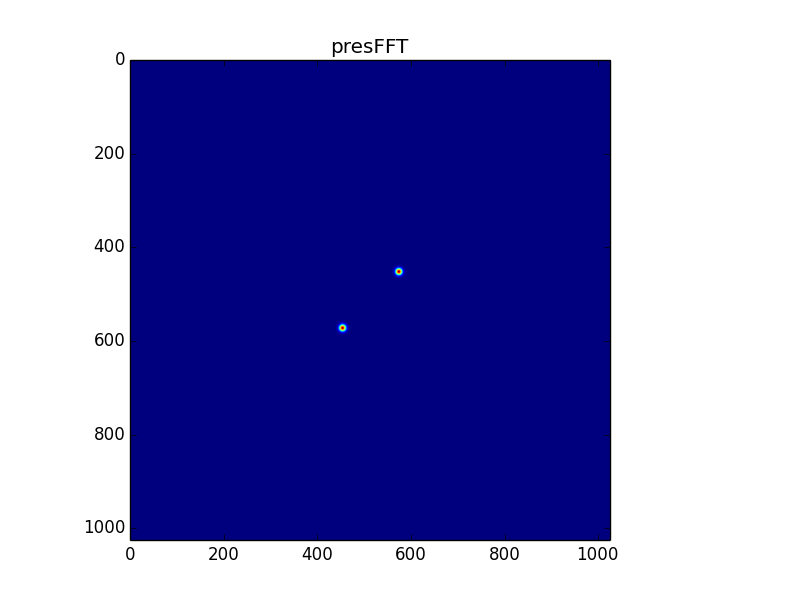
\includegraphics[scale=0.5]{fourier_ini.png}
 \caption{\emph{Fourier inicial (sin modificar los valores de los  coef ni las frecuencias según las expl de 1d)}}
\end{figure}


\paragraph{Ray tracing}
\begin{description}
\item determinar k(t) y x(t) de las ecuaciones diferenciales
\item k(t=0) =  $[K_0, K_1]$ , x(t=0) = $z_c$
\item calculamos en cada paso de tiempo k y x integrando las DE de arriba
\item podemos comprobar si k obtenido en cada paso de tiempo es igual a $k_c$ el valor donde la transf fourier tiene el máximo 


\item 
\item \textbf{Caso homogéneo}
\item k es constante $\implies$ las trayectorias son rectas

\item \textbf{Caso inhomogéneo} $cs(x) = cs(x_0) \implies k1 $ constante  
\begin{description}
\item $k_1 = 0$ las trayectorias son rectas, si cs crece en la dirección de k inicial , $k_0$ decrece, la componente en la direccion $x_0$ de las otras
componentes del paquete de ondas decrecen también y el paquete se abre
De forma similar si cs decrece en esta dirección, $k_0$ crece y el paquete se alarga
\item $k_0>0, k_1>0$ (el paquete va de izq arriba - derecha abajo), cs decrece en la direccion $x_0$ (arriba - abajo) , $k_0$ decrece y el paquete gira a la derecha

\end{description}


\end{description}

\paragraph{Videos}
\begin{description}
\item están en la carpeta videos. las simulaciones duran mucho y algunos tienen pequeños errores como en el caso de los  2 paquetes uno de los videos tiene la trayectoria de abajo calculada mal de forma analítica o el color de fondo que no queda constante (los límites del colormap en imshow). También debía haber guardado para cada simulación en la carpeta donde guardo las imagenes una copia de los ficheros *.py para saber exacatmente los parámetros de la perturbación , medio, condiciones de contorno,  esquema numérico,...
\end{description}


\end{document}


